% Chapter 1

\chapter{Hardware Implementation} % Main chapter title

\label{Chapter3} %

%----------------------------------------------------------------------------------------

\section{LeNet Pilot} \label{lenetpilot}

The main contribution in this work is in the form of a framework for the development and optimization of deep neural network operators on an FPGA. We use the Lenet \cite{lenet} model, knowing that it is outdated and outperformed by many other network architectures discussed before, due to its simplicity and as a pilot to test our framework. The simple network allows us to implement four different types of layers ( convolution, maxpooling, fully connected layers, and softmax). We also implement the backward propagation operators for all of the above layers.  We use LeNet to guide the numerous optimizations we perform on each layers separately and on the combination of the layers into a pipeline as well. We implement a modern variant of Lenet which only differs slightly from the original one. The first convolution in our model contains 10 feature maps as opposed to 6 in the original lenet\ref{fig:Lenet-5}, the second convolution outputs 20 feature maps as opposed to 15 feature maps. This adds more trainable parameters and thus we hope to use most of the MNIST dataset for training. For the sub-sampling layers we replace the average pooling operation by the maxpooling operation. We also use ReLU activation functions as opposed to the sigmoid as it has a lighter hardware implementaion and it has shown better results than the sigmoid in practice \cite{alexnet}. In the following sections we go more in detail about the implementation of the operators using OpenCL. 

\begin{table}[]
\centering
\begin{tabular}{ll}
\hline
\multicolumn{1}{|l|}{\textbf{Layer}} & \multicolumn{1}{l|}{ \textbf{No. Parameters}} \\ \hline
\multicolumn{1}{|l|}{C1}    & \multicolumn{1}{l|}{260}                            \\ \hline
\multicolumn{1}{|l|}{C2}    & \multicolumn{1}{l|}{5,020}                          \\ \hline
\multicolumn{1}{|l|}{C5}    & \multicolumn{1}{l|}{117,720}                        \\ \hline
\multicolumn{1}{|l|}{F6}    & \multicolumn{1}{l|}{10,164}                        \\ \hline
\multicolumn{1}{|l|}{\textbf{Total}}    & \multicolumn{1}{l|}{133,164}                        \\ \hline
\end{tabular}
\label{tab:custom-lenet}        
\caption{Number of Trainable Parameters for Custom LeNet Implementation}             
\end{table}


\section{Layer Implementations}

\subsection{Convolution Layer}

The fundamental operation in Convolutional Neural Networks is the convolution operation. This layer takes as input a multidimensional grid and extracts output feature maps by sliding a window of weights. The filter weights and biases are trainable by gradient descent. An output feature map pixel $ \mathit{y_{i}} $ is obtained by passing a filter of size $ K_{h}xK_{w} $ over an input feature $ \mathit{x_{i}} $ with $ \mathit{CH_{in}} $ input channels.
\begin{equation}
 y_{i} = relu(\sum_{c=0}^{c=CH_{in}} \sum_{h=0}^{h=K_{H}} \sum_{w=0}^{K_{w}} w_{i,c,h,w} * x_{c,h,w}  + bias_i ) 
\label{eqn:summat}
\end{equation}
The nested loop structure lends itself easily for parallelization.  We will discuss three different implementations for this layer and compare tradeoffs that can be used by the user 

\subsubsection{Simple Implementation with Unrolling} \label{simpleimpl}

With the help of high level synthesis, we can write a C-like implementation and analyze the performance. Assuming the kernel is pipelined we will require $ batch size * Img_h * Img_w * K_h * K_w * CH_{in} * CH_{out}  $ cycles theoretically to complete the convolution. To speed up the naive implementation we perform some optimizations:

\begin{itemize}
\item
\textbf{Unroll over filter computation}: Calculating each pixel in the output feature maps requires $ K_h * K_w * CH_{in} $ multiplications. As our filter sizes are small, we can unroll over the filter dimensions. By unrolling we are effectively parallelizing the algorithm by $ \mathit{25x} $ ( since in our case $ K_h = 5, K_w=5 $ ) . However, we choose to unroll over the input channels and the width of the kernel only. We choose input channels as opposed to only the kernel dimensions due to our memory layout because we stripe the input and  output feature maps by channels as the lowest rank dimension. This increases memory performance by performing batch aligned memory reads. 

\item
\textbf{Buffer the coefficients}: During the forward pass, the filter coefficients, will be read multiple times.  For that, we can reduce the amount of memory reads and buffer the coefficients in low-power and fast registers. This uses space on the board but allows us to access coefficients for a relatively cheaper cost.
\end{itemize}

Summations inside loops, such as in \ref{eqn:summat} can introduce memory dependencies as the result of the next iteration depends on a previous one. Memory dependencies get worse with unrolling factors as the critical path is increased. We carefully transfer the memory dependencies to local memory on the FPGA (discussed in more detail in \ref{loopdep} ) and achieve an ideal iteration index (ii) = 1. Therefore, the theoretical number of cycles for a convolution is expressed as 
\begin{equation}
Latency (L)  \approx ii * batch size * Img_h * Img_w * CH_{out} * K_h  \; cycles
\end{equation}

\lstinputlisting[style=CStyle, caption={code snippet from simple convolution}]{code/convPretty.c}


\subsubsection{Sliding Buffer Implementation} \label{slidingimpl}

In the simple implementation, we buffered the coefficients in low-cost local registers to avoid having to read the coefficients multiple times from memory. We also notice that when the convolution window slides with a stride of 1 step, there will be also values in the input feature map that are re-used. For that, we implement a sliding window that contain's all previously seen values as long as they can still be useful. Our implementation is similar to what is describe by Zohouri et. al \cite{2018combined}. The shift-register holds the input values and multiple taps allow for accessing the desired values in the sliding window. The intel offline compiler performs optimizations like replicating RAM blocks to allow for simulataneous access. For that, only few compiler directives should be specified to make this implementation work \ref{shiftinf}. This implementations is also an example of how we can trade local storage to minimize bandwidth. We also carry over the optimization done in the simple implementation.

\begin{figure}[h]
\centering
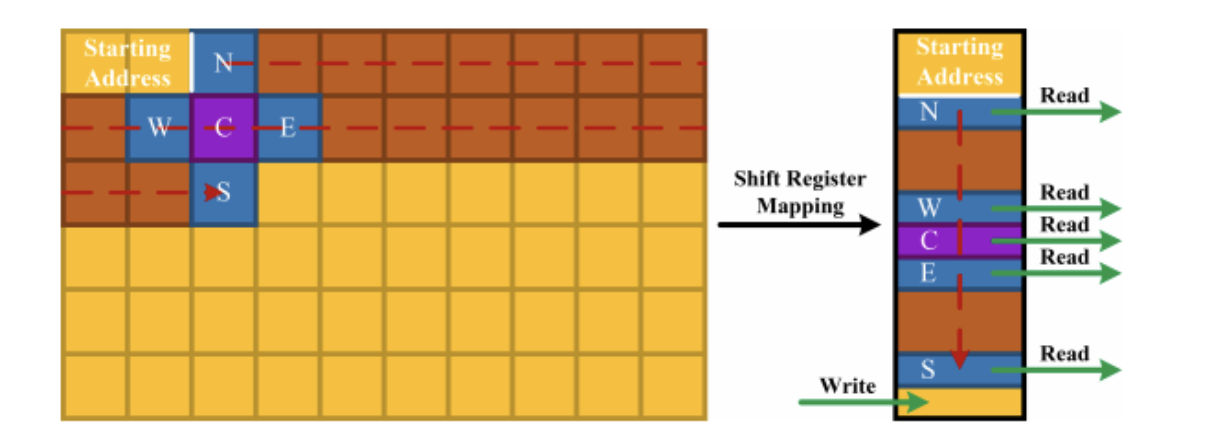
\includegraphics[width=0.6\textwidth]{Figures/slidingbuffer}
\decoRule
\caption[Sliding Buffer]{ Sliding Buffer Visualization. Source: \cite{2018combined}}
\label{fig:sliding buffer}
\end{figure}

\begin{figure}[h]
\centering
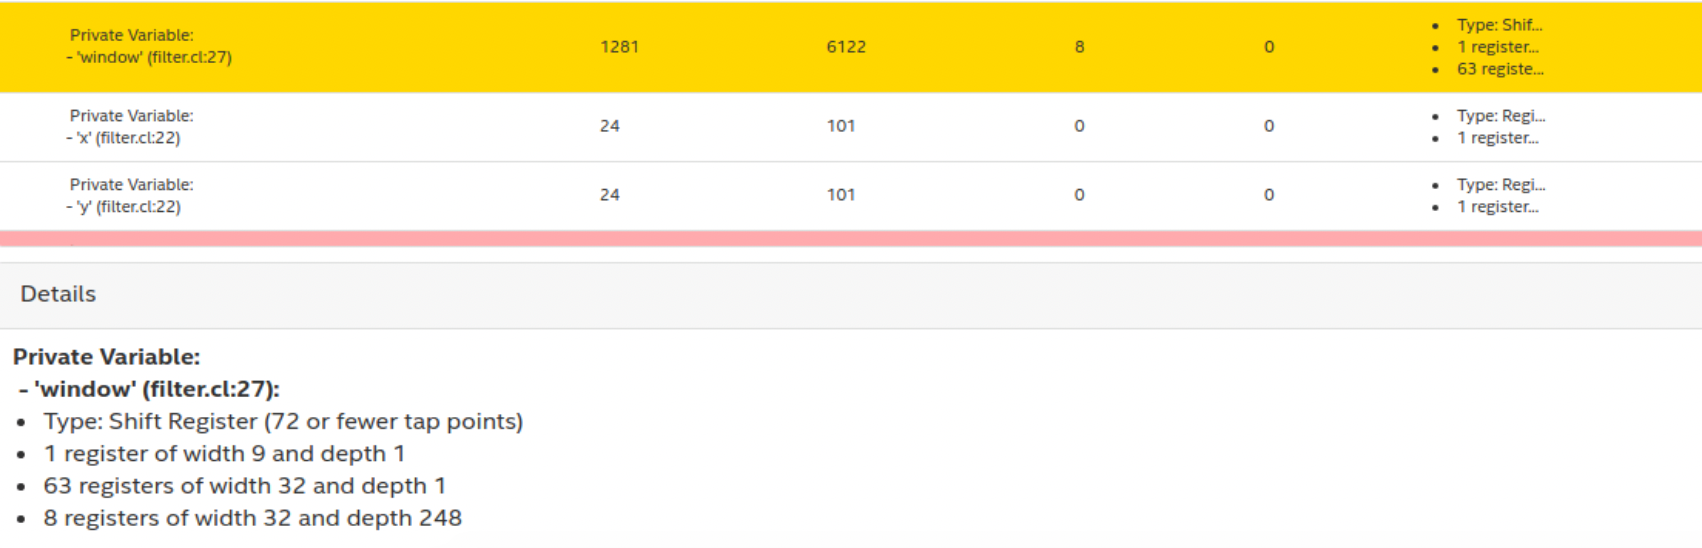
\includegraphics[width=1.0\textwidth]{Figures/shiftregister}
\decoRule
\caption[Shift Register]{ Sliding 'window' variable is inferred as a shift-register by the OpenCL compiler }
\label{fig:shiftregister}
\end{figure}

This implementation proves useful if data is provided in a streamlined fashion. The sliding buffer reads data sequentially and is more suitable for non-blocking dataflow computations.
\newline
\textbf{Limitations}
\newline
One of the limitations this implementation is that we quickly run out of buffer space as the dimensions of the problem grow larger. The sliding buffer size grows linearly with the above parameters: $ CH_{in}, Img_{w}, K_h, K_w $. For our application in a network as small as the Lenet, we do not worry about this problem. The solution to scaling the sliding buffer implementation is to utilize spatial blocking and tile the input into blocks and perform the computations in these tiles separately \cite{2018combined}.

\subsubsection{Row-stationary Implementation} \label{rowimpl}

\begin{figure}[h]
\centering
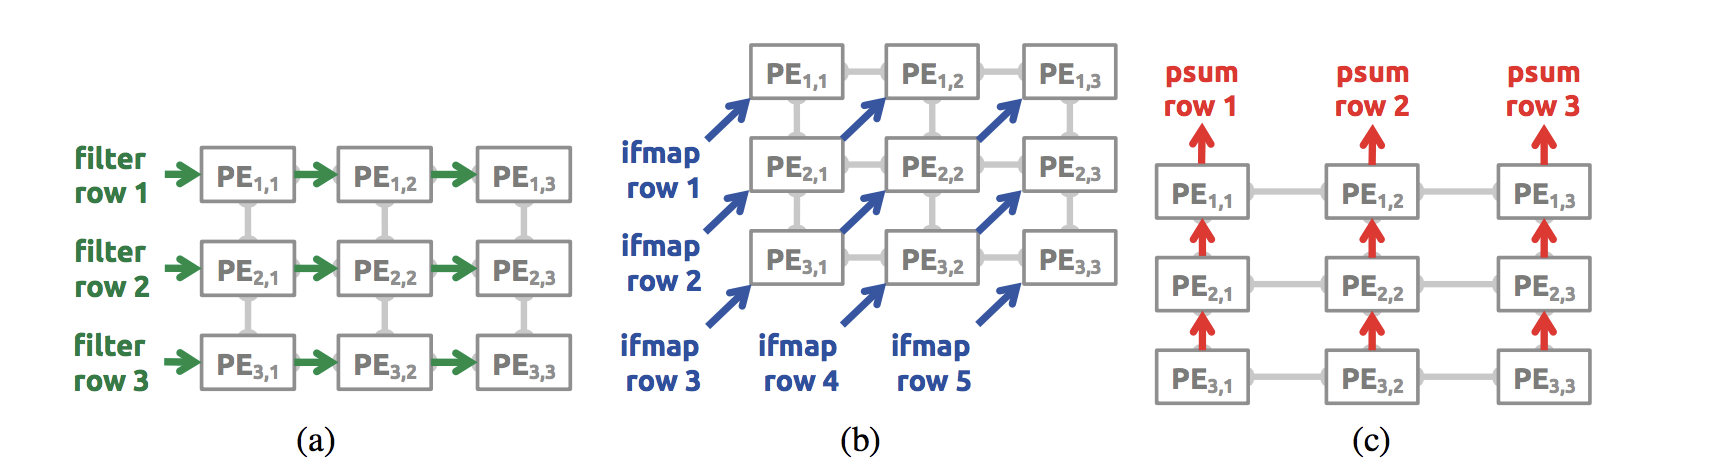
\includegraphics[width=1.0\textwidth]{Figures/eyeriss}
\decoRule
\caption[Data Re-use in Eyeriss]{ Datar re-use across processing elements in Eyeriss. Source: \cite{eyeriss}}
\label{fig:eyeriss}
\end{figure}

\begin{figure}[h]
\centering
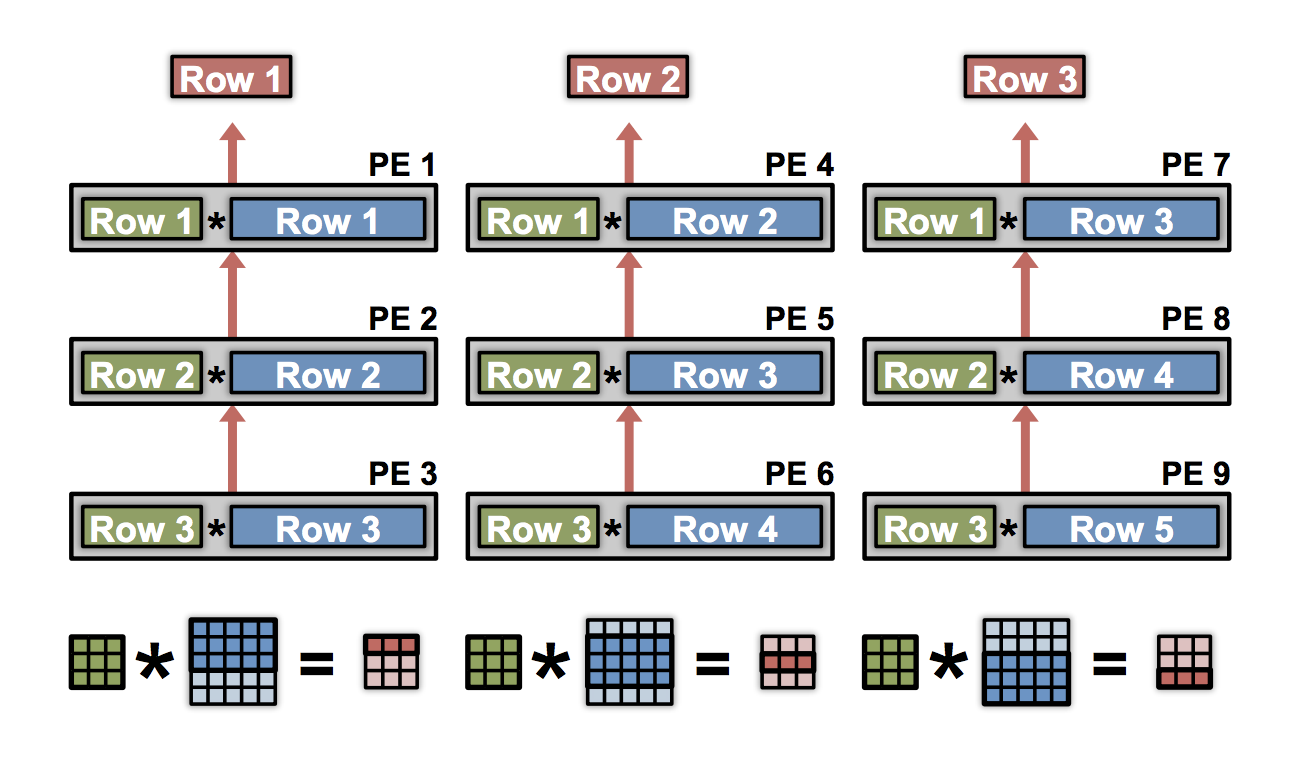
\includegraphics[width=0.6\textwidth]{Figures/eyeriss2}
\decoRule
\caption[2D Spatial Convolution]{ 2D spatial convolution with a grid of processing elements (Eyeriss). Source: \cite{sze2017efficient}}
\label{fig:eyeriss2}
\end{figure}

This approach was suggested by Chen. et. al \cite{eyeriss} and it presents a way of reusing both filter weights and input feature maps. The technique requires a set of replicated processing unit. In the simple case of 3x3 filters we can instantiate 9 processing elements (PEs) each holding one of the 3x3 filter weights \ref{fig:eyeriss}. We implemented a simplified version of this architecture using the Intel SDK’s autorun kernels, which means the kernels do not need to be explicitly invoked and can communicate data to each other using channels ( FIFOs ). Input feature maps are then streamed diagonally (blue \ref{fig:eyeriss}) where they are required for the computation of different output feature map rows. The partial sums are accumulated upwards vertically ( shown in red \ref{fig:eyeriss} ) upwards. 

Advantages of using this is that the size of this grid can be adjusted to best fit the resources available on a specific board. This dataflow performs the theoretical minimum of memory reads required as input fmaps are read once and communicated diagonally to other PUs based on demand. Communication between PEs is done through Intel OpenCL channels which are Intel’s implmentation of FIFOs ( or pipes in OpenCL terms ) and computations are performed asynchronously. Two separate reader and writer kernels handle reading and writing data between global memory and the processing grid. The size of this grid is reconfigurable and the user can instantiate a larger version of this grid. It is independant of the image and filter sizes as we reuse techniques from Eyeriss \cite{eyeriss} such as folding and replication to map different computations onto the same fixed grid.


\subsubsection{Other Implementations}

The below methods were \textbf{not implemented} but it is worth discussing other approaches to performing a convolution. The shared idea is to transform the convolution operation into another form of computation with different properties thus allowing to perform different types of optimizations. 

\textbf{Matrix Multiplication:} One solution to the convolution problem involves transforming the input matrix and incorporating redundant data as in \cite{cudnn}. This transforms the convolution operation into a direct matrix multiplication. The downside of using this is the requirement of either a larger storage for storing the redundant inputs or a very complicated memory access pattern to be implemented \cite{ddl}.

\textbf{Fast-Fourier Transform (FFT):} Another solution is found by transitioning into the Fourier domain and applying a fourier transform on both the filter and the input image \cite{vasilache2014fast}. In the Fourier domain, a convolution becomes again a matrix multiplication. After multiplication of the frequency domain representations of the filter and the input, we use the inverse-fourier transform to obtain the output image. The fourier-transform decreases the complexity of the convolution operation from $ O(N_o^2N_f^2) $ to $ O(N_o^2log_2(N_o) $ where the input image size is $ N_oxN_o$ and the filter size is $ N_fxN_f $ .The tradeoff in this case is less operations on the expense of additional bandwidth and storage requirements. The quality of this transformation and benefits degrade for smaller filters and thus fourier is usally used in the case when large input features and filters are required \cite{sze2017efficient}. 

\textbf{Strassen's Algorithm}\cite{cong2014minimizing}: can reduce the number of multiplications from $O(N^3)$ to $O(N^{2.8})$\cite{sze2017efficient} . The reduced multiplications lower the space requirement as floating point operators require more space than additions but comes at the expense of numerical stability and storage space requirement to hold and propagate intermediate results \cite{sze2017efficient}.

\subsection{Maxpool Layer}

\begin{figure}[h!]
\centering
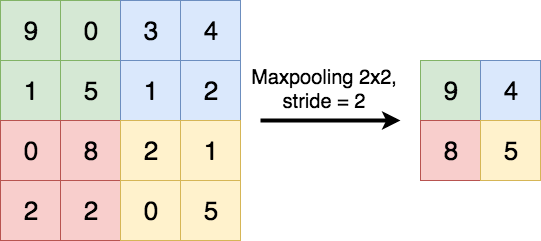
\includegraphics[width=0.5\textwidth]{Figures/maxpool}
\decoRule
\caption[maxpool]{ Maxpooling Operation}
\label{fig:maxpool}
\end{figure}

Convolution layers are usually followed by subsampling layers such as average pooling and maxpooling \cite{lenet}. These operations play a main role in decreasing the size of feature maps in the network and also add to the robustness and also make the network slightly shift-invariant and robust against distortions in the image \cite{alexnet}. Two common subsampling operations are the average pooling where the input values within a certain window are averaged and passed as one output feature map. The second type, which we choose to implement is the maxpooling which passes only the maximum value within a certain window in the input feature map to the output feature map. We developed two different implmentations for the maxpool operation which are the bandiwdth heavy, and streamlined version. 

\textbf{Bandwidth heavy:} the max operation within a certain window can easily be parallelized. In fact the maximum of the four values can be calculated in a single cycle and we can compute the one output pixel in the output feature map at a single clock cycle. Assuming we have sufficient bandwidth we can in fact perform the maxpool reduction to the whole input feature in one cycle however this requires reading the full feature map from memory at once which is impractical. For that, we limit the parallelization to the size of the window. In lenet, it is $ 2x2 $ which gives us a $ 4x $ speedup over the naive implementation of the sequential version of the problem. 

\textbf{Streaming calculation:} As we aim for efficiently pipelining the operators in a convolutional neural networks. We take into consideration the out input feature maps will be streamed in as an input. Therefore to perform the maxpool operation we should buffer in the whole first row and then we can proceed to produce the outputs sequentially. So assuming we are reading our data through an OpenCL channel, the way to fix this is to borrow from the already implemented solution for the sliding buffer convolution. In fact, the maxpool operation iterates over an ifmap as a convolution however in our case the stride size is equal to the filter dimensions $ 2x2 $. We adapt the sliding buffer implementation from the convolution layer to the maxpool layer and use it in our generic maxpool template. 

\subsection{Non-Linearities} 

In between convolution layers and fully connected layers, non-linear functions are applied on the output feature maps. Without non-linear functions, a neural network ( no matter how many layers it consists of ) would behave as a single layer perceptron because summing the layers would give just another linear function. We implement both classical non-linearities such as the sigmoid function and the hyperbolic tangent, in addition to the ReLU function. The ReLU non-linearity  define as $ relu(x)  = max(0, x) $ has proven to increase accuracy \cite{alexnet}, in addition to accelerating training as the derivative can be simply coded as $ relu'(x) = 1 $ if $ (x \geq 0 ) $ else $ 0 $ .  In terms of hardware the relu derivative is simply a MUX wired to constant values of 0 and 1. We implement these operations as a streamlined operation which is pipelined with an $ ii $ of 1.

\subsection{Softmax}

For the output layer we implement the \emph{Softmax} operation. It can be used as a modular output layer for a network that performs multi-class classification such as the LeNet. The operation is defined as follows: 
\begin{equation}
	f(z_j) = \frac{e^{z_j}}{\sum_{k=1}^{K} e^{z_k} } \hspace{1cm}  \mbox{\emph{for j=1,...,K}}
\end{equation}
and it is used to map K outputs to K possible probability values in a categorical distribution. This function highlights the maximum values and suppresses those that are a certain order of magnitude below the maximum value.  Due to the interdependency for normalizing the outputs, the softmax needs to read all output values before it operates, however the operation is unrolled, and since this is the final layer the output of this operation is written directly to memory.

\subsection{Backpropagation}

Backpropagation for all of the layers in the above sections. We summarize all backpropagation kernels in one section for two reasons; the first being that backpropagation operators borrow the same implementation from the forward calculations.i.e backprop of a convolutional layer is also a convolution, and backprop of a fully connected layer is also a matrix multiplication. We believe that the main challenge introduced by implementing backpropagation is that It requires additional buffer space to hold intermediate outputs. For that we are faced with two options:
\begin{itemize}
\item
Replicate writes in the pipeline to global memory and find a way to synchronize forward and backward operations.
\item
Use kernels that read and write to memory and run them sequentially and then eventually run backpropagation.
\end{itemize}

\begin{figure}[h]
\centering
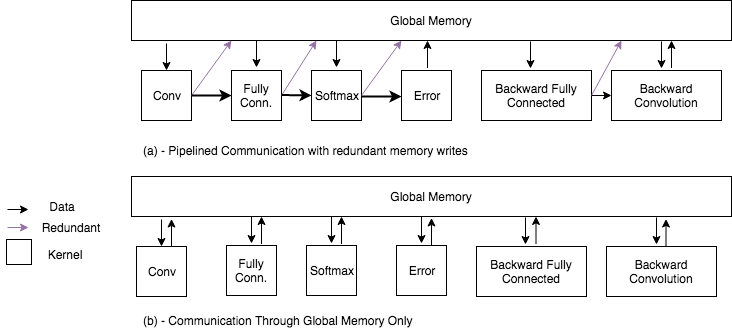
\includegraphics[width=0.9\textwidth]{Figures/comm}
\caption[Types of inter-layer communication]{ Two types of inter-layer communication }
\label{fig:comm}
\end{figure}

We choose to go with option (b) in training neural networks, though not optimal, due to time limit constraints. Our backpropagation algorithm is not pipelined only due to the fact that we need to store intermediate results and this makes it easier as a first prototype for training neural networks on FPGAs. This only impacts performance slightly, because when kernels communicate through memory several parallelization techniques can be performed while sacrificing bandwidth. Also as each kernel runs in a separate timeslot, the whole board bandwidth is available for the single layer which offers us more flexibility in parallelization and making use of the maximum bandwidth. Another thing to note is that profiling kernels is easier and we can better see the time consumed by each kernel and relieve bottlenecks for different operators or architectures 

Backpropagation is the process of propagating an an error back to the network layers in order to adjust the weights. The gradient is propagated backwards in the network based on the chain rule in differential calculus. Several weight update rules ranging from a fixed learning rate to adaptive and momentum-based methods are explored in literature \cite{ddl}. In our implementation we keep the learning rate as an input argument so that it can be configured at runtime by the host program. This allows for flexibility in experimenting with different weight update rules without the need to rebuild the kernel.

The trainable weights are usually initialized to small random values in the range $ (-0.5,0.5) $. In practice, the random weights are then normalized depending on the weight activations used\footnote{\url{https://medium.com/usf-msds/deep-learning-best-practices-1-weight-initialization-14e5c0295b94} Last Accessed: 25/08/2018}. There are also different weight normalization schemes used in practice to mitigate ( but not completely solve ) problems that arise in deeper networks like the vanishing or exploding gradient \cite{hochreiter1998vanishing}. For the ReLu activation, it is common to multiply the random weights by a factor of $ \sqrt{\frac{2}{sizeof(prev. layer)}} $. This initialization is done on the host side and the weights are then transferred to the FPGA in the beginning of the training procedure. 


\begin{figure}[h]
\centering
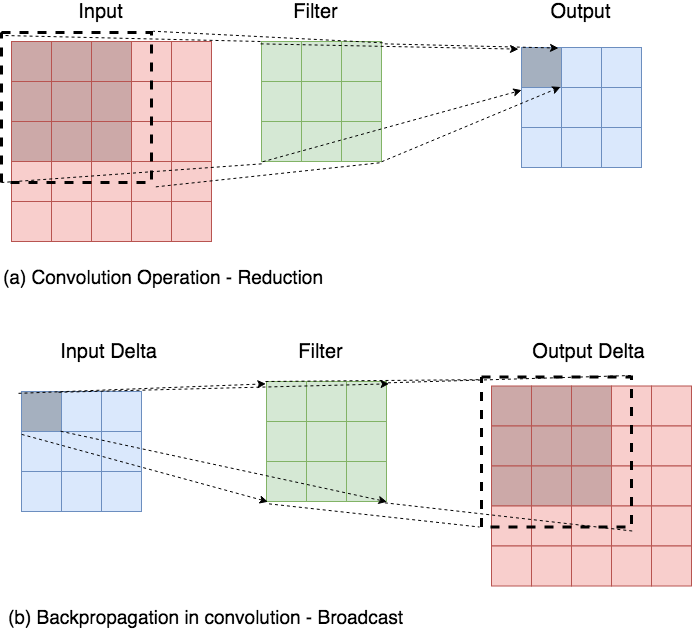
\includegraphics[width=0.6\textwidth]{Figures/convprop}
\caption[Propagation of data in convolution]{ Propagation of data in convolution }
\decoRule
\label{fig:conv}
\end{figure}

\textbf{Convolution Backpropagation:} The backpropagation of a convolution operator is also a convolution. For that we borrow some optimizations performed on the forward convolution such as buffering the coefficients, and unrolling over kernel dimensions. We note the main difference is that in inference phase, a window of dimensions $ K_wxK_h $ is sliding along an input feature map in order to obtain an output feature map. Thus this is more of a \emph{reduction} performed by multiply and accumulation of values in a specific window. In the case of propagating back an error, the input delta ( coming from the output feature map ) is \emph{broadcast} to all of the pixels in the input feature maps ( also show a picture here ). A simple implementation would introduce memory dependencies on calculations, another way is to rearrange dimensions and use local buffering to hold values of the output deltas before writing to memory. The backpropagation kernel we implemented is fully pipelined with $ ii=1 $ and also performs batched weight updates for the filters.

\textbf{Maxpool backpropagation:} For backpropagation through maxpool, we simply pass upstream the error to the input pixel in a certain window with the maximum value. The same implementation from the forward max pooling is used with the addition of passing an output gradient at the maximum as opposed to passing the maximum value downstream. In our case the maxpool does not have any trainable parameter and acts as a multiplexor that passes down the error as it is. 

\textbf{Fully connected backpropagation:} The fully connected layers used for classification contain most of our trainable parameters. In the case of minibatches we use a matrix multiplication technique for both forward and backward propagation of the error. We also try to unroll computation loops to utilize the maximum bandwidth available for this kernel. The backpropagation is a similar inverse computation ( still matrix multiplication)  and the weights are also updated according to a configurable learning rate.

\textbf{Loss}: For the loss function we implemented a cross entropy loss function (\ref{tab:loss}). It measures divergence of the softmax output probabilities ( representing a categorical distribution ) with the target output probabilities as a \emph{one-hot} encoding.

\section{OpenCL Kernel Template Generator}

Many parameters such as sliding window sizes, kernel size, and number of input and output channels should be known at compile time. Each of the discussed layers is parametrized by a specific set of parameters that it takes in as a configuration. For that we created a python tool that instantiates instances  given a kernel template in ‘.cl’ format ( the extension for OpenCL kernels). The idea is to use a configuration file in JSON to customize a specific layer. In conjunction, we used a python library called jinja2\footnote{\url{http://jinja.pocoo.org/docs/2.10/} Last Accessed: 25/08/2018} to instantiate templates.Templating allows us to instantiate multiple versions of the kernel to be used and compiled together for the neural network accelerator.


\begin{figure}[h!]
\centering
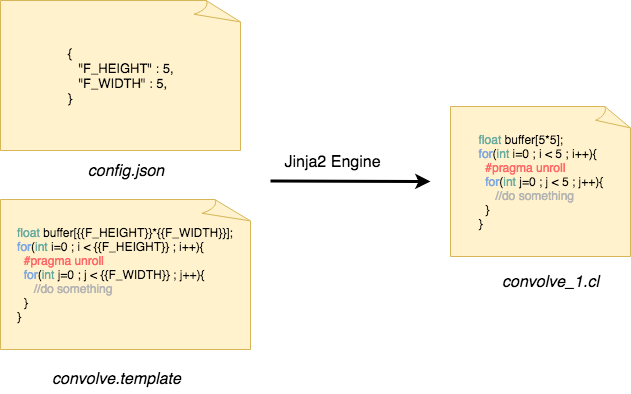
\includegraphics[width=0.9\textwidth]{Figures/jinja}
\decoRule
\caption[Templating Kernels]{ Templating Kernels }
\label{fig:jinja}
\end{figure}

\begin{figure}[h!]
\centering
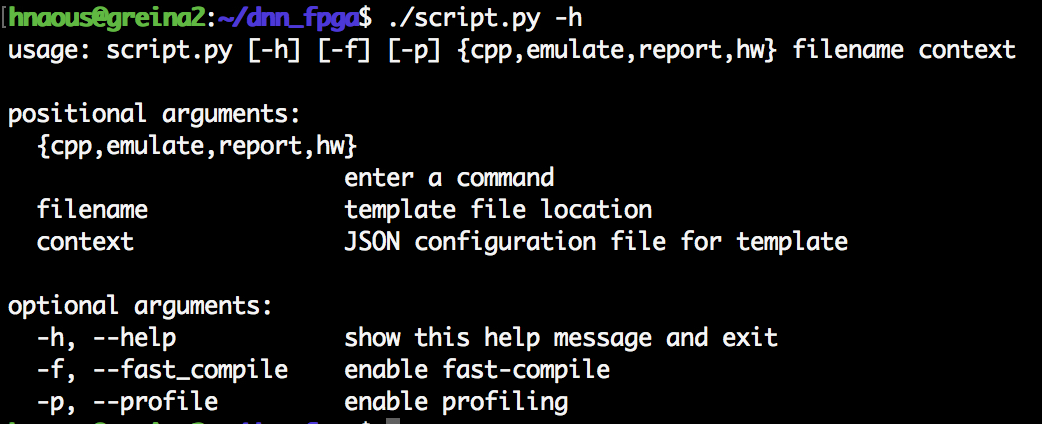
\includegraphics[width=0.7\textwidth]{Figures/usage}
\decoRule
\caption[Tempate Generator Usage]{ OpenCL Template Generator Usage }
\label{fig:usage}
\end{figure}

The basic usage is exposed through the interface shown in \ref{fig:usage}. The Python tool allows the user to also perform additional tasks on the generated kernel such as generating the performance report, compiling for emulation, compiling for hardware, and compiling the kernel as a as a C++ application using gcc. We discuss the use of compiling   as a C++ application in section 5(REF HERE). This type of compilation differs from the traditional workflow suggested by Intel as we have extended the emulation framework of kernels and use C++ to perform unit testing and verifying correctness of the operators. This rids us from the responsibility of creating a host program that interfaces with the kernel and from a lot of overhead code in managing the device buffers just for the sake of verification. 
As for the additional functions such as generating report, and compiling for hardware, the additional value provided by the tool is that it supports instantiating multiple templates at the same time and combining them in a single report or a single binary. All of the kernel implementations discussed in \ref{Chapter3} are designed as templates and the generator tool is used for instantiation, and interaction with the Intel compiler to perform different types of analysis.

\section{Integration with Deep500}

Deep500\footnote{\url{https://github.com/deep500} Last Accessed 25/08/2018} is a library developed internally in the Scalable and Parallel Computing Lab at ETH to aid in the process of developing custom backends for computational graphs. It enables the extension of operators, verification, network optimization, and acts as a distributed learning framework for deep neural network models. The networks are expressed in ONNX\footnote{\url{https://github.com/onnx/onnx} Last Accessed : 25/08/2018 } format. ONNX is an open source format to represent computational graphs ( specifically deep neural networks ). It allows the interoperability between different deep learning frameworks such as torch\cite{torch} and tensorflow\cite{tensorflow} and the exchange of models and parameters in between those frameworks for performing optimizations, training, and inference. 

\begin{figure}[h!]
\centering
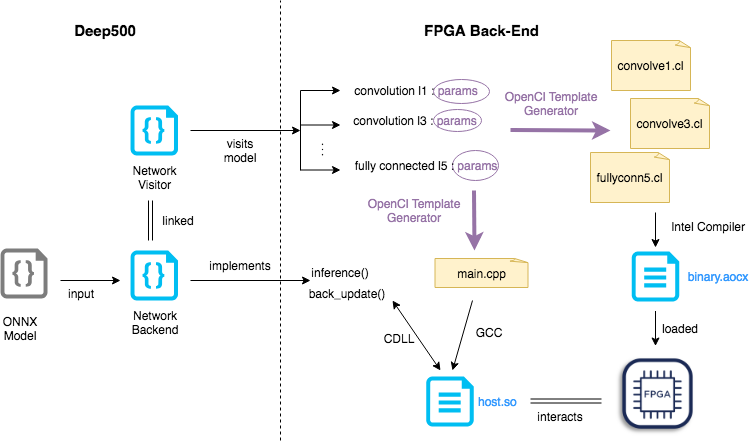
\includegraphics[width=1.0\textwidth]{Figures/integration}
\decoRule
\caption[Intergration with Deep500 Diagram]{ Custom FPGA Back-End for ONNX Models }
\label{fig:integration}
\end{figure}

The Deep500 library provides us with an extendable visitor interface to implement each of the operators required for a given onnx model. For example in our network, the operations we implement are convolution, maxpooling, relu, and gemm ( generalized matrix multiplication ). The Deep500 library traverses the model’s operations using a NetworkVisitor class. We extend the visitor class to implement all of the mentioned operations. Each visit to a node in the graph provides the parameters and input shapes required for implementing this node's operation. We use those parameters to instantiate an OpenCL kernel using the template generator we created. With the \emph{.cl} files available, we are able to transform an ONNX model into a group of inter-related OpenCL kernels that can be built for hardware \ref{fig:integration}. From there we can use again the tool to view the area utilization report, emulate the kernel, and perform additional unit tests on each of the operations.
To enable training and inference using the kernels and built CL files, we require a host program running on the CPU that interacts with the above kernels. The host program is in C++ and has to be customized for the computational graph it runs. For that we choose to template the host program also using  \emph{jinja2}. In addition, we also use the operation parameters to be able to generate a suitable host program.  
\emph{jinja2} allows us to use nested JSON configurations and arrays in order to generate the host program. The host program performs the following operations : setting up opencl environment, passing data between the host program and the FPGA's global memory buffer, and enqueuing kernels to be executed on the FPGA.

For the accelerator backend to work it should communicate with the templated host program, so after instantiating the host program, we compile it as a shared object \emph{'host.so'}. This allows us to use python’s CDLL library to create a handle to the C++ program. The forward and backward propagation functions are exposed externally to CDLL and we can easily pass down coefficients and inputs to the host program,which executes and returns the results.

The added value and end result of this work is given an ONNX model we can create and compile the relevant FPGA binaries by using Deep500 to traverse the graph. We are also able to instantiate and compile a controller host program, and interact with this host program to train a neural network. The benefit also extends to other popular DNN frameworks where models can be exported to onnx. For example the pytorch library offers the option of exporting torch models to onnx, the implementation offers the ability to interact with this tool and train other networks on an FPGA. It is also worth mentioning that  Deep500 allows us to perform unit-tests to verify each of the implemented operations on the FPGA.

%-----------------------------
